\documentclass[a4paper]{article}
\usepackage[OT1]{fontenc}
\usepackage{Sweave}
\usepackage{url}
\usepackage{afterpage}
\usepackage{hyperref}
\usepackage{geometry}
\geometry{ hmargin=3cm, vmargin=2.5cm }
\usepackage{graphicx}


\begin{document}

% \VignetteIndexEntry{a4vignette}

\title{Using the \texttt{a4} package}
\author{Willem Talloen, Tobias Verbeke}

\maketitle

\tableofcontents
\pagebreak{}



\section{Preparation of the Data}
First we load the package \texttt{a4} and the example real-life data set \texttt{ALL}.
\begin{Schunk}
\begin{Sinput}
R> library(a4)
R> data(ALL, package = "ALL")
\end{Sinput}
\end{Schunk}

For illustrative purposes, simulated data sets can also be very valuable (but not used here).
\begin{Schunk}
\begin{Sinput}
R> require(nlcv)
R> esSim <- simulateData(nEffectRows = 50, betweenClassDifference = 5, 
     nNoEffectCols = 5, withinClassSd = 0.2)
\end{Sinput}
\end{Schunk}

\subsection{ExpressionSet object}
The data are assumed to be in an expressionSet object. Such an object structure combines different sources
of information into a single structure, allowing easy data manipulation (e.g., subsetting, copying)
and data modelling.

The texttt{featureData} slot is typically not yet containing all relevant
 information about the genes.
This interesting extra gene information can be added using \texttt{addGeneInfo}.

\begin{Schunk}
\begin{Sinput}
R> ALL <- addGeneInfo(ALL)
\end{Sinput}
\end{Schunk}


\subsection{Some data manipulation}
The \texttt{ALL} data consists out of samples obtained from
two types of cells with very distinct expression profiles; B-cells and T-cells. To have a more subtle signal,
gene expression will also be compared between the BCR/ABL and the NEG group within B-cells only.
To this end, we create the expressionSet \texttt{bcrAblOrNeg} containing only B-cells with BCR/ABL or NEG.
  
\begin{Schunk}
\begin{Sinput}
R> Bcell <- grep("^B", as.character(ALL$BT))
R> subsetType <- "BCR/ABL"
R> bcrAblOrNegIdx <- which(as.character(ALL$mol) %in% 
     c("NEG", subsetType))
R> bcrAblOrNeg <- ALL[, intersect(Bcell, bcrAblOrNegIdx)]
R> bcrAblOrNeg$mol.biol <- factor(bcrAblOrNeg$mol.biol)
\end{Sinput}
\end{Schunk}

\pagebreak{}
\section{Unsupervised data exploration}

Spectral maps are very powerful techniques to get an unsupervised picture of how the data look like.
A spectral map of the \texttt{ALL} data set shows that the B- and the T-subtypes cluster together along the
 x-axis (the first principal component).
 The plot also indicates which genes contribute in which way to this clustering. For example, the genes located
 in the same direction as the T-cell samples are higher expressed in these T-cells. Indeed, the two genes at the
  left (TCF7 and CD3D) are well known to be specifically expressed by T-cells (Wetering 1992, Krissansen 1986).
 
\begin{Schunk}
\begin{Sinput}
R> spectralMap(object = ALL, groups = "BT")
R> legend("bottomright", legend = levels(pData(ALL)$BT), 
     text.col = a4palette(nlevels(pData(ALL)$BT)), 
     bty = "n")
\end{Sinput}
\end{Schunk}
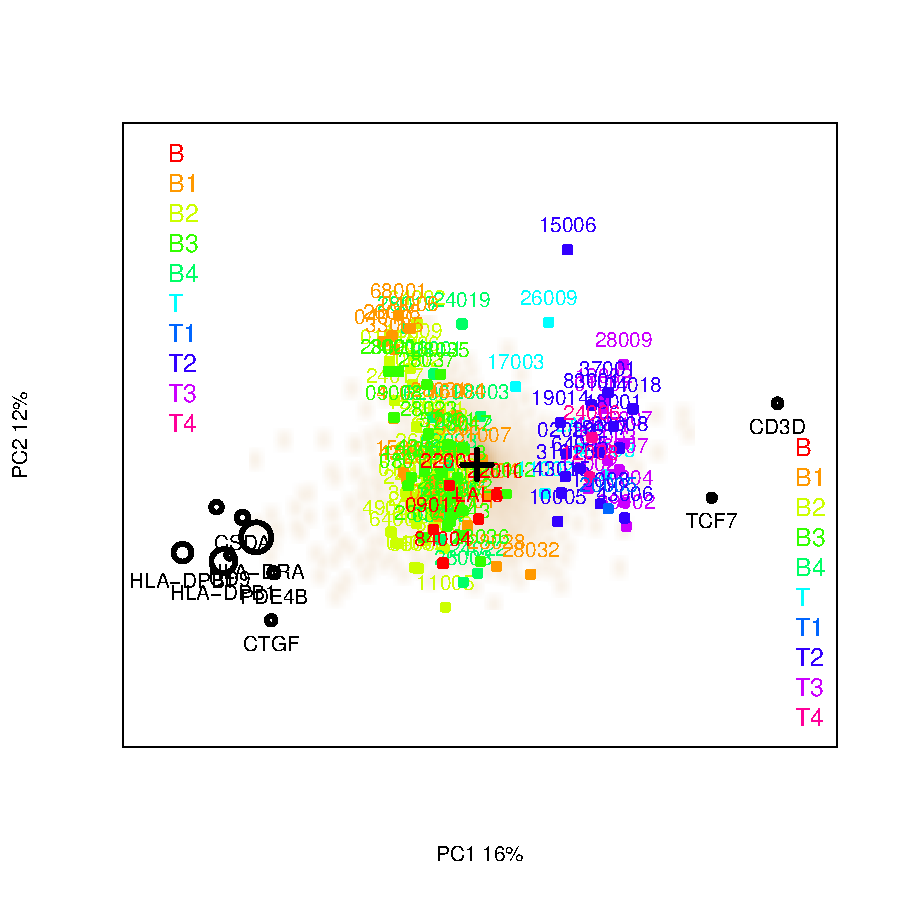
\includegraphics{a4vignette-spectralMapALL}

A spectral map of the \texttt{bcrAblOrNeg} data subset does not show a clustering of BCR/ABL or NEG cells.

\begin{Schunk}
\begin{Sinput}
R> spectralMap(object = bcrAblOrNeg, groups = "mol.biol", 
     probe2gene = TRUE)
R> legend("topright", legend = levels(pData(bcrAblOrNeg)$mol.biol), 
     text.col = a4palette(nlevels(pData(bcrAblOrNeg)$mol.biol)), 
     bty = "n")
\end{Sinput}
\end{Schunk}
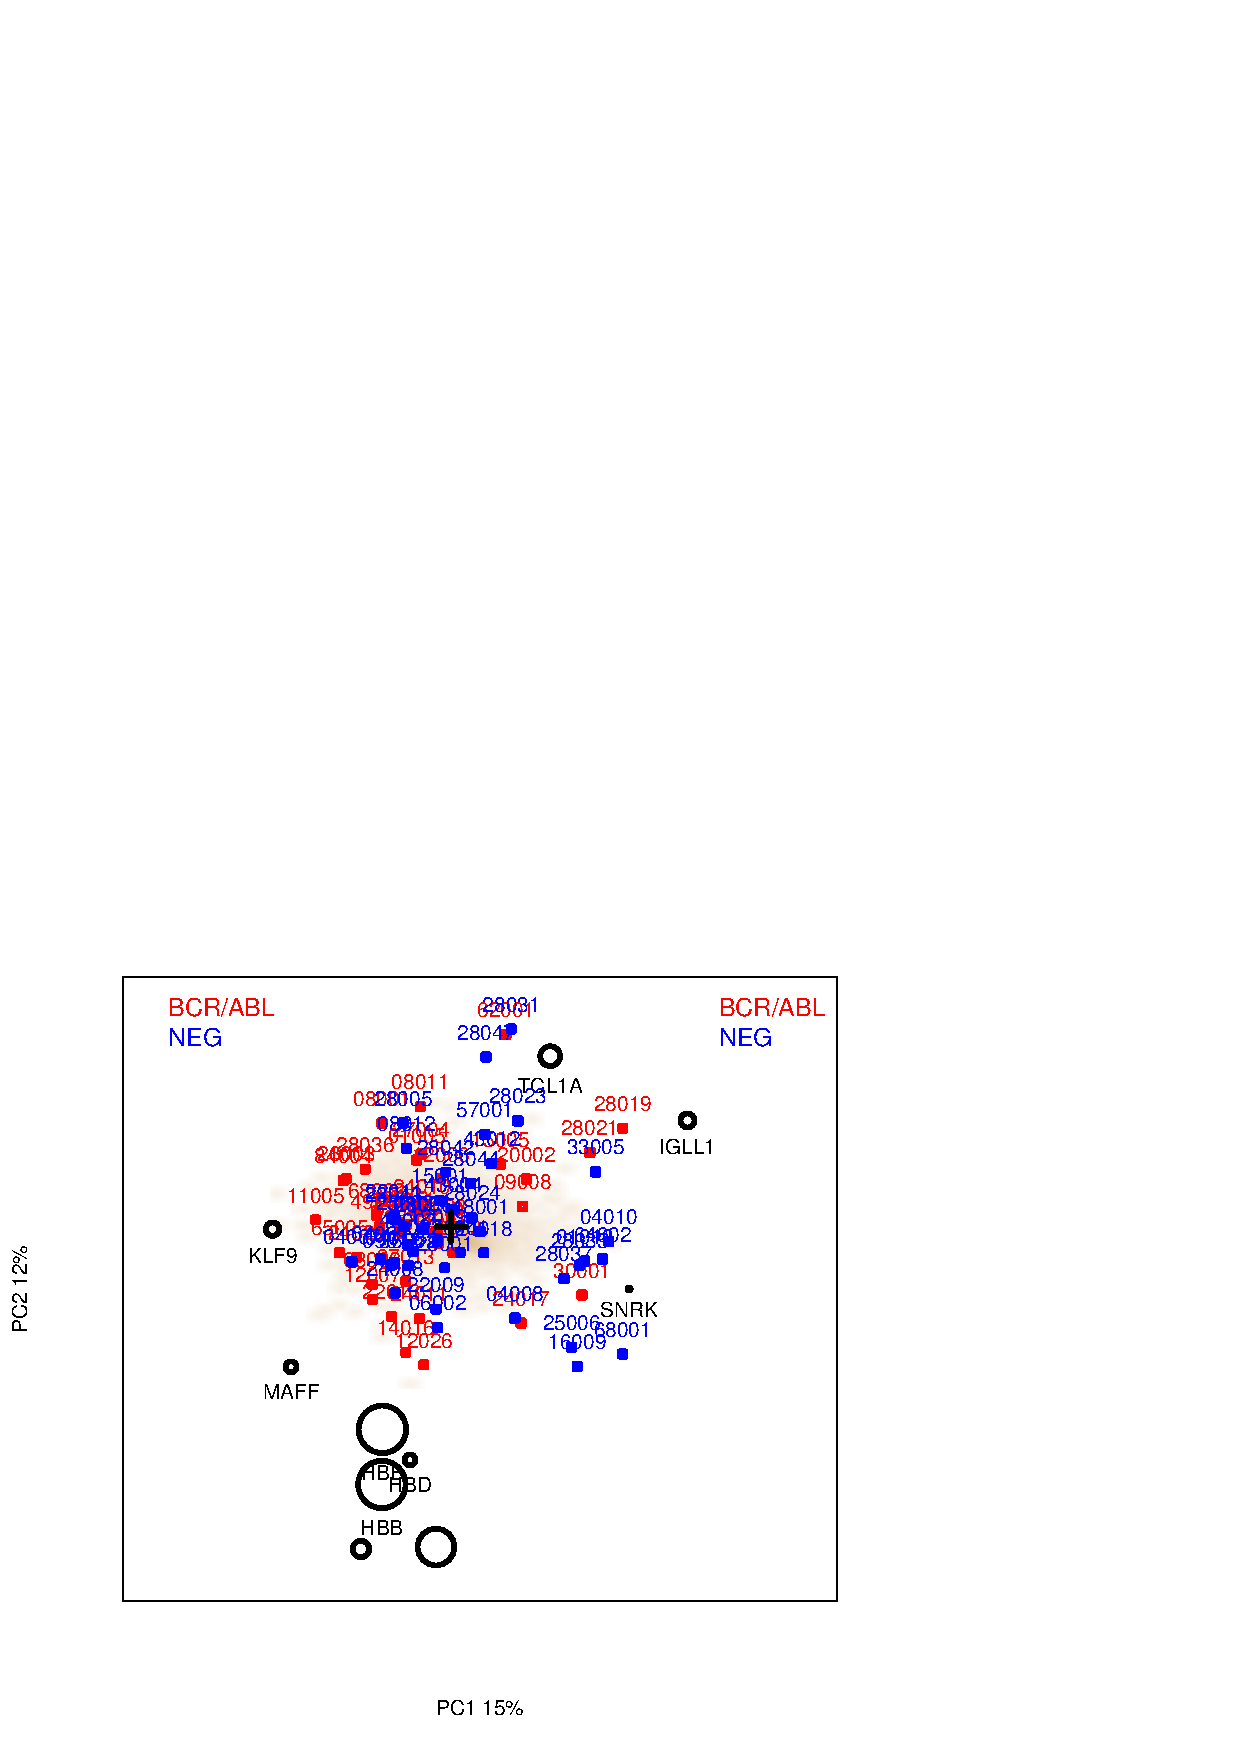
\includegraphics{a4vignette-spectralMapALLSubset}

\section{Filtering}
The data can be filtered, for instance based on variance and intensity, in order to reduce
 the high-dimensionality.

\begin{Schunk}
\begin{Sinput}
R> selBcrAblOrNeg <- filterVarInt(object = bcrAblOrNeg)
R> propSelGenes <- round((dim(selBcrAblOrNeg)[1]/dim(bcrAblOrNeg)[1]) * 
     100, 1)
\end{Sinput}
\end{Schunk}

This filter selected 18.9 \% of the genes
(2391 of the in total 12625 genes).

\pagebreak{}
\section{Detecting differential expression}

\subsection{T-test}

\begin{Schunk}
\begin{Sinput}
R> tTestResult <- tTest(selBcrAblOrNeg, "mol.biol")
\end{Sinput}
\end{Schunk}
\begin{Schunk}
\begin{Sinput}
R> histPvalue(tTestResult[, "p"], addLegend = TRUE)
R> propDEgenesRes <- propDEgenes(tTestResult[, 
     "p"])
\end{Sinput}
\end{Schunk}
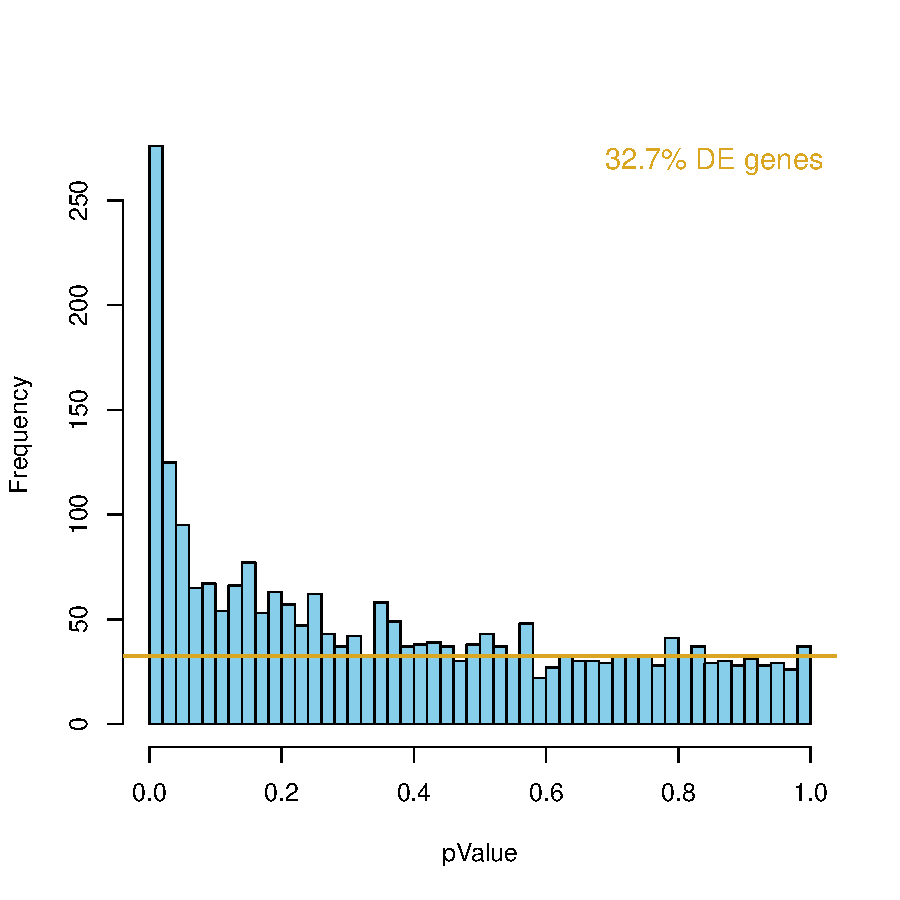
\includegraphics{a4vignette-tTestHist}

Using an ordinary t-test, there are 171 genes significant at a FDR of 10\%.
The proportion of genes that are trully differentially expressed is estimated to be around 32.7.

The toptable and the volcano plot show that three most significant probe sets all target \texttt{ABL1}.
This makes sense as the main difference between BCR/ABL and NEG cells is a mutation in this particular ABL gene.

\begin{Schunk}
\begin{Sinput}
R> tabTTest <- topTable(tTestResult, n = 10)